\subsection{Realizing \ogs{} with MicroNet}

\begin{figure}
	\centering
	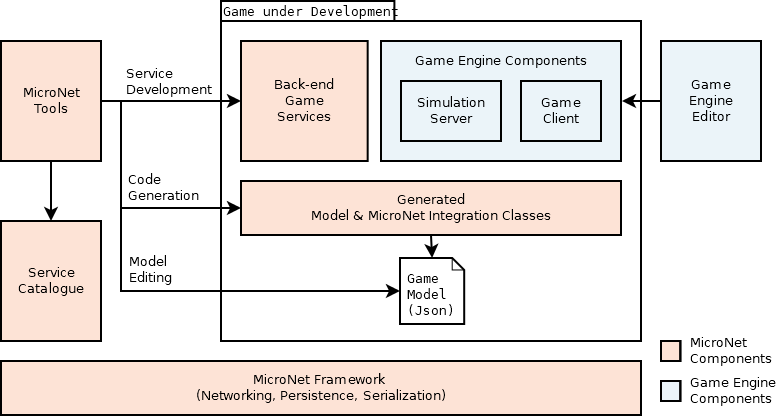
\includegraphics[width=\textwidth]{images/architecture/GameWithMicroNet}
	\caption{The MicroNet setup for \og{} development.}
	\label{fig:game_with_micronet}
\end{figure}

\autoref{fig:game_with_micronet} shows how the MicroNet development setup for an
\og{} looks like. The game model is represented by \gls{json} files and is used
to generate the classes needed to participate in a MicroNet application. This
allows the integration of the back-end game services but also of the game
simulation server and the client into the application. Back-end can also bypass
the generated integration layer and directly use the framework functionality.

The game engine components are developed using the game engines regular
development workflow. The integration of MicroNet can be achieved by either
mirroring the framework integration generation in the language of the game
engine or manually program the integration classes.

A disadvantage of this setup is that the framework integration layer has to be
realized for all used technologies. This introduces quite an overhead but is
compensated by the improved work-flow which is possible once the integration is
done. It has to be mentioned that the implementation effort to realize the code
generation part which generates the framework integration classes is rather
small. The model definition and editing take care of most work in this regard.
The code generation layer is only responsible to generate simple classes out of
the well defined \gls{json} model files which is a very doable task and well
documented through the MicroNet code generation plug-in which serves as a
reference implementation. Also the developer has always the choice to integrate a foreign
technology into MicroNet by using only ActiveMQ as the message broker bypassing
the integration layer. ActiveMQ is very portable since it offers many clients on
many platforms.

With the integration layer out of the way the developer is free to use the
MicroNet tools to speed up and clarify the development process. This includes
the possibility to integrate reference services from the service catalogue into
the application. It also includes the possibility to use MicroNet core
features like networking, persistence, and serialization.
